\chapter{Antecedentes}

\section{Fatiga}
El fenómeno en el cual una estructura se daña e incluso falla por cargas fluctuantes, es llamado fatiga. El estudio de este problema comenzó tempranamente en europa durante la mitad del siglo XIX, en pleno auge de la industralización europea, producto de la falla repentina de algunos componentes en máquinas y los ejes de los trenes de la época. Estos experimentaban un gradual debilitamiento de la resistencia, fallando aún cuando su esfuerzo último no fuese alcanzado. 

Así, en 1837 fueron publicados los resultados del primer ensayo de fatiga, realizado a una cadena transportadora utilizada en minas de hierro en Alemania. Wilhelm Albert, quien realizó esta investigación, se vió motivado a realizar los estudios por los altos costos que significaba la falla de este componente producto de las cargas cílicas a las que estaba sometida. Los pocos conocimientos existentes del fenómeno en esa época, llevo a que la solución al problema fuese la invención del cable de acero.

Por otro lado, las primeras investigaciones enfocadas a comprender el fenómeno comenzaron en 1858 con August Wölher. Su acucioso estudio lo llevó a conclusiones que siguen teniendo importancia y validez hasta el día de hoy. Diseñó, durante la década de 1860, una máquina de ensayos de flexión y flexión rotativa. En 1870 presentó un informe en el cual parte de sus conclusiones cualitativas son llamadas ``Ley de Wöhler'', al establecer el esfuerzo alternante como el parámetro más importante para la vida de un componente, señalanado que ``the stress amplitudes are decisives for the destruction of the cohesion of the material. The maximum stress is of influence only in so far as the higher it is, the lower are the stress amplitudes which lead to failure''\textcolor{red}{citar schutz history of fatigue}, aunque destacando también que el esfuerzo medio tiene una influencia perjudicial en el material. 

Es decir, desde 1853 hasta hoy, han transcurrido más de 160 años de investigación sobre la fatiga, logrando comprender distintas aristas del fenómeno, pero con muchas preguntas aún sin resolver. Por eso, la fatiga sigue siendo un problema necesario de abordar y seguir comprendiendo, por sus grandes implicaciones de costo que tiene en la industria y en distintos elementos que utilizamos en la vida diaria. Por otro lado, si bien muchas preguntas no han sido resueltas científicamente, diversas empresas han logrado evitar las fallas por fatiga y optimizar los diseños de manera operativa, sin comprender cabalmente el trasfondo de estos.

\subsection{Medición de la fatiga}
Existen distintas técnicas para cuantificar la respuesta de un material o componente frente a esfuerzos o deformaciones fluctuantes. La primera de ellas, como se habló anteriormente, corresponde a una viga giratoria sometida a flexión en voladizo, diseñada por A. Wöhler. Con respecto a la información existente en la literatura la mayoría de los datos disponibles de resistencia a la fatiga se encuentra en las pruebas de viga giratoria (\textit{rotating bending}, en inglés) en ciclo de flexión invertida, seguido por cargas axiales (\textit{push-pull}, en inglés), flexión en voladizo (\textit{alternating bending}, en inglés) y en menor medida, en las pruebas de fatiga por torsión. \textcolor{red}{citar norton seccion 45}

\subsubsection{Ensayo de fatiga con una viga giratoria en flexión} 
Su uso es el más extendido para determinar la vida a fatiga de un material. La principal ventaja frente a otros sistemas radica en su capacidad de aplicar ciclos de cargas a altas velocidades, es decir, realizar pruebas de fatiga a altas frecuencias. Sin embargo, no es posible aplicar una carga media distinta de cero, por lo tanto, su uso principal se encuentra en la obtención de datos para el rango HCF y de ciclo invertido. Los datos obtenidos son más altos respecto a otros tipos de medición, como se puede ver en la figura REF.


\subsubsection{Ensayo de fatiga axial}
Esta configuración de prueba es más flexible que el resto, siendo posible cualquier combinación de esfuerzo alternante y medio, además de poder realizar ensayos con el modelo de deformación-vida. Su principal diferencia respecto al método de viga giratoria se encuentra en que la sección transversal está sometida a esfuerzos de manera uniforme, provocando que los resultados de resistencia a la fatiga obtenidos sean usualmente menores que las obtenidas por \textit{rotating bending} y \textit{alternating bending}. Se considera que esto se debe a la  probabilidad más alta de hallar una microgrieta en un campo de esfuerzos más grande. Asimismo, la superposición de momentos de flexión sobre las cargas axiales, producto de la dificultad de crear cargas axiales sin excentricidad, son un factor en la disminución en la obtención de valores de resistencia menores. En concreto, la reducción de las resistencias a la fatiga obtenidos pueden variar entre un 10$\%$ y un 30$\%$ o más si hay flexión producto de la excentricidad de las cargas. La figura REF \textcolor{red}{sacar imagen de paper A Esin} muestra las diferencias de los datos obtenidos entre un ensayo de fatiga axial y uno de viga giratorio.

\subsubsection{Ensayo de fatiga de flexión en voladizo}
Esta prueba consiste en someter a una viga en voladizo a oscilaciones en su extremo libre a través de algún mecanismo, pudiendo lograr combinaciones de esfuerzos medios y alternantes. La máquina analizada en esta memoria, utiliza este método para la obtención de los datos de vida de fatiga del material a analizar. Los resultados de este tipo de prueba son inferiores a los obtenidos por \textit{rotating bending} y mayores a los obtenidos por \textit{push-pull}.

\subsection{Correlación entre distintos métodos de medición de la fatiga}
Como se señaló anteriormente y se aprecia en la imagen REF, cada prueba entrega valores distintos aún cuando los niveles de esfuerzo sean iguales. Por esto, existen distintos intentos en la literatura de crear correlaciones entre los datos, evitando los costos asociados a realizar nuevos ensayos experimentales del mismo material o componente. La forma en que se ha abordado esta problemática es la utilización de un factor de corrección ($\phi$) calculado con distintas propuestas.

Algunos de estos modelos son: Manson y Muralidharan, Philipp, Lee y Esin. Cada metodología aborda de distinta forma el cálculo del factor de corrección $\phi$, ahora bien, se abordarán los modelos de Lee y Esin en este trabajo, ya que, de acuerdo a \textcolor{red}{agregar cita de analysis of axial papre}, son los modelos que se ajustan mejor al comportamiento de los datos empíricos entre ensayos de \textit{rotating bending} y de \textit{push-pull}. \textcolor{red}{corregir}

\subsubsection{Modelo de Esin}
El modelo propuesto por Esin en \textit{``A method for correlating different types of fatigue curve"}, relaciona las curvas $S$-$N$ de los ensayos \textit{push-pull}, \textit{alternating bending} y \textit{rotating bending}. Éste depende del esfuerzo alternante, asumiendo que la curva base y la calculada por este método se intersectarán en el punto ($S_e,N_f$), es decir, el factor de correción es $\phi=1$ en esa posición. 

El método se basa en el análisis de la dependencia de la micro-plasticidad en la distribución de esfuerzos en la sección transversal, definiéndose la micro-plasticidad como el flujo plástico de un material sin haber alcanzado su punto de fluencia. Ésta ocurre sobre cierto nivel de esfuerzos en el rango elástico, llamado límite elástico real (\textit{true elastic limit}, en inglés o \textit{TEL}) y bajo el límite de resistencia a la fatiga, $S_e$. Así, siempre se cumplirá que:
\begin{align*}
	\text{\textit{TEL}} \leq S_e \leq S_y
\end{align*}

La micro-plasticidad es un fenómeno altamente localizado que depende de las propiedades probabilísticas micro-estructurales del material como su micro-inhomogeneidad, anisotropía y micro-concentraciones de esfuerzos, los cuales explican la dispersión de datos en los ensayos de fatiga. Así, cuando los esfuerzos alternantes están sobre valor del  \textit{TEL}, la micro-plasticidad influye en los macro-elementos. Dicho de otra forma, el comportamiento mecánico observado a un nivel macro es el comportamiento integrado de los micro-elementos.

\textcolor{red}{Hacer imagen igual a esta}
\begin{figure}[h]
\centering
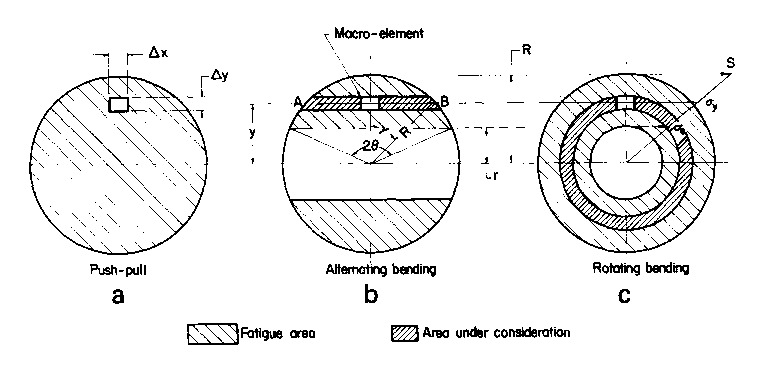
\includegraphics[scale=1]{Imagenes/affectedarea_fatigue.pdf}
\caption{Sección transversal de probetas sujetas a esfuerzo alternante uniaxial. \textit{a) push-pull}, \textit{b) alternating bending} y \textit{c) rotating bending}}
\label{fig:affar_fat}
\end{figure}

En la figura \ref{fig:affar_fat}, se puede apreciar las áreas afectadas por fatiga para cada tipo de ensayo, los cuales, por sí mismo podrían explicar las diferencias en los resultados de cada prueba. Sin embargo, basándose en el criterio de fatiga de la deformación micro-plástica, la falla ocurre cuando la energía acumulada por la histérsis plástica, a una cantidad de ciclos $N_f$, es igual al valor de la energía de ruptura real (área bajo la curva de un diagrama $\sigma$-$\varepsilon$ real), como queda expresado en la ecuación \ref{eq:nfail_esin}.

\begin{equation}\label{eq:nfail_esin}
	N_f = \frac{U \cdot T_t}{W} 
\end{equation}

Donde:
\begin{itemize*}
	\item $N_f$: Número de ciclos a la falla.
	\item $U$: Energía total real bajo la curva del diagrama esfuerzo-deformación.
	\item $W$: Energía total plástica disipada.
	\item $T_t$: Número total de macro-elementos.
\end{itemize*}

De esta forma, el método utiliza varios factores para crear una correlación entre las distintas curvas, ocupando el esfuerzo alternante, $S$, como valor de entrada. El primero de ellos es el concepto de esfuerzo alternante equivalente, $S_{eq}$ (ecuación \ref{eq:esfalt_eq}), utilizado para denotar un esfuerzo hipotético actuando sobre todos los elementos sometidos a fatiga. 
\begin{equation}\label{eq:esfalt_eq}
	S_{eq} = \frac{\Sigma \sigma_i A_i}{\Sigma A_i}
\end{equation}
Donde $A_i$ es el número o área de los macro-elementos con igual esfuerzo equivalente. A partir de esto, el esfuerzo equivalente para ensayos de \textit{rotating bending} y \textit{alternating bending}, están dados por las ecuaciones \ref{eq:seq_rotben} y \ref{eq:seq_altben}, respectivamente. 
\begin{align}
	S_{eq,rt} &= \frac{2S\cdot \sin^3 \theta}{3C} \label{eq:seq_rotben}\\
	S_{eq,ab} &= \frac{2S}{3} \cdot \left(\frac{1-c^3}{1-c^2}\right) \label{eq:seq_altben}
\end{align}
Donde las variables $C$ y $c$ se definen cómo:
\begin{equation}
	C= \left(\frac{\pi\theta}{180} - \frac{\sin(2\theta)}{2}\right)\qquad ;\qquad c=\frac{r}{R}
\end{equation}
Los valores de $\theta$, $r$ y $R$ son propios de la geometría de la probeta utilizada y se definen de acuerdo a la figura \ref{fig:affar_fat}. De igual forma, se debe calcular el factor de fatiga, $FF$, ecuación que representa el ratio entre el área total de la sección transversal y el área de los elementos que contribuyen al proceso de fatiga. Así, las ecuaciones \ref{eq:ff_ab} y \ref{eq:ff_rb} representan los factores de fatiga para calcular la vida a fatiga equivalente, $N_{eq}$, de \textit{alternating bending} y \textit{rotating bending}, respectivamente.
\begin{align}
	FF_{ab} &= \frac{\pi}{2} \left(\frac{\pi\theta}{180} - \frac{\sin(2\theta)}{2}\right) \label{eq:ff_ab}\\		
	FF_{rb} &= \frac{R^2}{(R^2 - r^2)} \label{eq:ff_rb}
\end{align}
Finalmente, con estos elementos es posible tomar del diagrama $S$-$N$ un punto ($S_i$,$N_i$) y, a través de las correlaciones, obtener un nuevo punto ($S_i'$,$N_i'$) que equivale a la curva $S$-$N$ de otro tipo de ensayo.

La metodología consiste en tomar un valor de esfuerzo alternante conveniente $S$ y calcular su esfuerzo alternante equivalente, $S_{eq}$. Utilizando este valor, se determinará a partir de la curva $S$-$N$ original el número de ciclos a la falla que se llamará vida a fatiga equivalente, $N_{eq}$. Este valor debe ser multiplicado por el factor de fatiga $FF$, obteniendo la vida a fatiga modificada, $N$. Así, el punto $P=(S,N)$, como se muestra en la figura REF \textcolor{red}{Crear fig 3 del paper de Esin} es el valor equivalente obtenido, teniendo que repetirse el procedimiento para todos los puntos que se requieran.

\subsubsection{Modelo de Lee}
La estimación del límite de fatiga, $S_e$, se calcula a través de distintos factores de modificación según el tipo de carga, calidad superficial, tamaño y confiabilidad de la muestra. El factor de modificación según el tipo de carga $C_L$ varía entre 0,7 y 0,9 para probetas sin muescas. Las recomendaciones para cada valor de $C_L$ se realizaron considerando los efectos del gradiente de esfuerzos y el tipo de esfuerzo involucrado, es decir, cortantes y normales. Estos también varían según el tipo de material, los cuales fueron obtenidos de manera empírica. Así la tabla \ref{tab:lee_factor} muestra los factores de modificación para algunos tipos de carga.

\begin{table}[h]
\centering
\begin{tabular}{@{}llc@{}}
\toprule
Tipo de Carga                & $C_L$ & \multicolumn{1}{l}{Observaciones} \\ \midrule
Carga axial pura             & 0,9   & -                                 \\
Carga axial con leve flexión & 0,7   & -                                 \\
Rotating bending             & 1,0   & -                                 \\
Torsional                    & 0,58  & \multicolumn{1}{l}{Para aceros}   \\ \bottomrule
\end{tabular}
\caption{Factores de modificación por tipo de carga, según el modelo de Lee.}
\label{tab:lee_factor}
\end{table}

Además, es posible apreciar en la imagen REF \textcolor{red}{hacer imagen como la 416 del texto de Lee pag 150} las diferencias que se generan por la aplicación del factor de corrección para los distintos tipos de carga que se buscan. 

AÑADIR IMAGEN COMPARANDO AMBOS SISTEMAS.

\section{Máquina de fatiga a flexión}
El desarrollo de este trabajo se centrará en la máquina de fatiga que posee el departamento de ingeniería mecánica en el laboratorio de tecnología mecánica en Valparaíso. La información existente sobre la máquina de ensayo es escasa principalmente por su antigüedad, lo que ha llevado a la perdida de documentos y la obsolescencia de la tecnología de la parte eléctrica.  

A partir de la información verbal entregada por el profesor Guillermo González, la máquina fue adquirida por el departamento durante la década del 50. Fue fabricada en Suiza por \textit{Alfred J. Amsler \& Co.} y su estructura completa es de acero fundido. Previo a la remodelación del piso del laboratorio durante el año 2012, la máquina se encontraba montada sobre un colchón de corcho, que a su vez se anclaba a un bloque hecho de concreto. Este fue demolido durante los trabajos, momento desde el cual se encuentra apoyada sobre la mesa de madera sin una solución definitiva. Más aún, varios equipos y máquinas de ensayo del laboratorio no se encuentran ancladas al piso ni con una instalación definitiva, impidiendo su correcto uso.

La máquina consiste, en un primer acercamiento, en un disco desequilibrado de forma controlada por el usuario, el cual, al ser acelerado angularmente hasta una velocidad definida por su motor eléctrico, comienza a oscilar. Esta oscilación es transmitida, a través de un brazo de carga, hacia la probeta en forma de momento. La probeta se encuentra doblemente empotrada, por un lado está fija a la estructura de la máquina y, por el otro, empotrado al brazo de carga que le realiza el momento. Los elementos que generan el desequilibrio son pequeñas masas calibradas, como se puede apreciar en la imagen \ref{fig:contrapesos}, que se denominarán contrapesos. La máquina también entrega la posibilidad de realizar ensayos de fatiga a torsión, al girar los empotramientos 90 grados, sin embargo, esta configuración no se estudiará en este trabajo. Un estudio a mayor profundidad se realizará en la sección \ref{sec:lev_info}.

\section{La madera como elemento constructivo}
La madera es un material de construcción simple y liviano, con ciertas características que lo vuelven particular respecto a otros materiales de construcción. Esto hace que al momento de trabajar con la madera se requiera un conocimiento especial y se tomen en consideración reglas específicas que permitan realizar diseños de calidad que aprovechen al máximo las propiedades y beneficios que provee.

Existen cientos de variedades de madera, donde cada una tiene propiedades distintas. Además, al haber sido parte de un organismo vegetal en crecimiento, hace que ninguna pieza de madera sea igual a otra y, dependiendo del tipo de corte, también varíen las propiedades mecánicas. Frente a esta importante variabilidad del material, surgen las normas en cada país que intentan delimitar y clasificar las distintas especies madereras que se encuentran en su región según el tipo de corte, contenido de humedad, su calidad o uso. Incluso, existen distintas metodologías de cálculo si se utiliza madera maciza, laminada encolada o aglutinada. En el caso de este trabajo, se utilizará exclusivamente madera maciza, por lo tanto, toda la metodología de cálculo e información respectiva a este tipo de madera, a excepción del pino radiata, se encuentra en la norma NCh 1198 Of - Madera - Construcciones en madera - Cálculo.

\subsection{Anatomía de la madera}
La madera es un material que es fabricado naturalmente por los vegetales leñosos, con un alto grado de especialización y complejidad. Esto lo vuelva altamente heterogéneo, al estar especializado en llevar a cabo las funciones fundamentales del vegetal, lo que se ve reflejado en sus propiedades físicas y mecánicas. 

Una consecuencia de esta heterogeneidad es el comportamiento anisotrópico, teniendo un comportamiento distinto según la dirección en que se trabaja. Se establecen tres planos de referencia respecto a su propiedades físicas.
\begin{itemize}
	\item Longitudinal: Sigue la misma dirección de la fibra o el eje del tronco.
	\item Radial: Pasa por el eje del tronco y es perpendicular a los anillos de crecimiento.
	\item Tangencial: Paralela a un plano tangente a los anillos de crecimiento.
\end{itemize}
En relación a sus propiedades mecánicas se habla de dos direcciones, la paralela (longitudinal) y normal o perpendicular (englobando radial y tangencial). Esta diferencia hace que la madera sea capaz de soportar cargas de compresión de hasta 4 veces en dirección paralela respecto a la normal. Esto quiere decir que siempre que sea posible, se deben instalar las piezas madereras para que resistan las cargas en su dirección longitudinal para un uso eficiente del material. De esta forma, se habla que las propiedades mecánicas de la madera son ortotrópicas.

Por último, es considerado un material higroscópico por su capacidad de captar o ceder agua del exterior, tanto en forma líquida como vapor. La cantidad de agua que contiene tenderá a estar en equilibrio con su entorno, lo que afectará sus propiedades físicas, mecánicas y en su posible degradación.

\subsection{Propiedades mecánicas de la madera}
Junto a la ortotropía de la madera, existen otras particularidades que influyen en sus propiedades, como la duración de la carga, el contenido de humedad y su calidad. En el primer caso, dado su carácter orgánico, es susceptible a degradarse por elementos externos como la lluvia, hongos, insectos o el sol protegiendola a través de tratamientos químicos, e internos, que se expresa en un factor de modificación por duración de carga para . En el segundo caso, a mayor cantidad de humedad la resistencia comienza a decaer, como también sus dimensiones se comienzan a modificar, afectando las uniones o ensambles. En último término, la calidad se reflejada en la cantidad de nudos, desviaciones de fibra o gemas que influyen en su comportamiento.

La tracción y compresión tienen resistencias distintas, además de las diferencias existentes entre las cargas paralelas y perpendiculares a la madera. La resistencia a la tracción paralelamente es comúnmente más alta que la compresión paralela, en la cual se debe calcular además la inestabilidad lateral. En el caso de la compresión y tracción perpendicular, los valore de resistencia son considerablemente más bajos, llegando a ser 9 y 20 veces menos resistente que su par paralelo, respectivamente. Esto se debe a la eficiencia de construcción de los árboles al no estar solicitados fuertemente en estas direcciones. 

Esta diferencia de resistencia y comportamiento entre la tracción y compresión de la madera implica que en el cálculo de la flexión se deban separar las zonas flexo-comprimidas y flexo-traccionadas, a pesar que la resistencia a la flexión de una madera sea única. Por otro lado, los esfuerzos cortante en un elemento de madera puede tener diversos modos:
\begin{itemize}
	\item Cortadura: las fibras son cortadas transversalmente.
	\item Deslizamiento: las fibras se desplazan longitudinalmente.
	\item Rodadura: las fibras se desplazan una sobre otra.
\end{itemize}
Donde la rotura se produce por deslizamiento al ser el plano más débil.

En última instancia, la resistencia a la fatiga de la madera es muy buena en comparación a otros materiales estructurales con estructura cristalina como el acero\textcolor{red}{citar libro guia de madera}, siendo resistente a la acción cíclica de las cargas y al amortiguamiento de estas. 

\section{Acero}
El acero es una aleación basada principalmente en fierro y carbono, pudiendo tener concentraciones de otros elementos incluso. Sus propiedades mecánicas son fuertemente sensitivas al contenido de carbono, por lo que muchas veces es clasificado a partir de su porcentaje, como aceros de bajo, media y alto en carbono.

La probeta utilizada en la máquina de fatiga se fabrica actualmente de acero de bajo carbono, los cuales bajo nomenclatura AISI/SAE se denominan 1020 y 1040, es decir, son aceros que sólo contienen concentraciones residuales de otros elementos distintos al carbono y su concentración es del 0,20\% y 0,40\% respectivamente.

Los aceros de bajo carbono se caracterizan por ser más débiles, pero con una alta tenacidad. Además, son maquineables, soldables y más baratos respecto a otros tipos de aceros. 



